% main=manual.tex

\section{Drawing axes and plots}
\subsection{\TeX-dialects: \LaTeX, Con{\TeX}t, plain \TeX }
\label{sec:tex:dialects}%
\PGFPlots\ is compatible with \LaTeX, Con{\TeX}t and plain \TeX. The only difference is how to specify environments. This affects any \PGF/\Tikz-environments and all \PGFPlots-environments like axis, semilogxaxis, semilogyaxis and loglogaxis:
\begin{description}
\def\HEAD{%
	\small
	\lstset{boxpos=b,breaklines=false,aboveskip=3pt,belowskip=3pt}%
	%\hspace{-1cm}%
	\begin{tabular}{*{2}{p{4cm}}}%
}%
\item[\LaTeX:] \lstinline!\usepackage{pgfplots}! and

{\HEAD
\begin{lstlisting}
\begin{tikzpicture}
\begin{axis}
...
\end{axis}
\end{tikzpicture}
\end{lstlisting}
&
\begin{lstlisting}
\begin{tikzpicture}
\begin{semilogxaxis}
...
\end{semilogxaxis}
\end{tikzpicture}
\end{lstlisting}
\\
\end{tabular}%
}

A small \LaTeX--example file can be found in
\begin{lstlisting}
doc/latex/pgfplots/pgfplotsexample.tex.
\end{lstlisting}

\item[Con{\TeX}t:] \lstinline!\usemodule[pgfplots]! and

{\HEAD
\begin{lstlisting}
\starttikzpicture
\startaxis
...
\stopaxis
\stoptikzpicture
\end{lstlisting}
&
\begin{lstlisting}
\starttikzpicture
\startsemilogxaxis
...
\stopsemilogxaxis
\stoptikzpicture
\end{lstlisting}
\\
\end{tabular}%
}

A small Con{\TeX}t--example file can be found in
\begin{lstlisting}
doc/context/pgfplots/pgfplotsexample.tex.
\end{lstlisting}

\item[plain \TeX:] \lstinline!\input pgfplots.tex! and

{\HEAD
\begin{lstlisting}
\tikzpicture
\axis
...
\endaxis
\endtikzpicture
\end{lstlisting}
&
\begin{lstlisting}
\tikzpicture
\semilogxaxis
...
\endsemilogxaxis
\endtikzpicture
\end{lstlisting}
\\
\end{tabular}%
}

A small plain--\TeX--example file can be found in
\begin{lstlisting}
doc/plain/pgfplots/pgfplotsexample.tex.
\end{lstlisting}
\end{description}
You may need to set low--level drivers if you intend to use \texttt{dvipdfm}, see section~\ref{sec:drivers}.

\subsection{A first plot}
Plotting is done using \lstinline|\begin{axis} ... \addplot ...; \end{axis}|:

\begin{figure}
\centering
\begin{tikzpicture}
	\begin{axis}[
		xlabel=Cost,
		ylabel=Error]
	\addplot[color=red,mark=x] coordinates {
		(2,-2.8559703)
		(3,-3.5301677)
		(4,-4.3050655)
		(5,-5.1413136)
		(6,-6.0322865)
		(7,-6.9675052)
		(8,-7.9377747)
		(9,-9.9717663)
	};
	\end{axis}
\end{tikzpicture}

\caption{An example for a normal plot. Here, coordinates are specified using the \Tikz-syntax ``\texttt{plot coordinates}'', optional labels can be provided with the ``\texttt{xlabel}'' and ``\texttt{ylabel}'' arguments.}
\label{fig:firstplot}
\end{figure}

\begin{lstlisting}
\begin{tikzpicture}
	\begin{axis}[
		xlabel=Cost,
		ylabel=Error]
	\addplot[color=red,mark=x] coordinates {
		(2,-2.8559703)
		(3,-3.5301677)
		(4,-4.3050655)
		(5,-5.1413136)
		(6,-6.0322865)
		(7,-6.9675052)
		(8,-7.9377747)
		(9,-9.9717663)
	};
	\end{axis}
\end{tikzpicture}
\end{lstlisting}
The outcome of this listing is shown in figure~\ref{fig:firstplot}. The \lstinline!plot coordinates! command is one of the \Tikz\ ways to create plots, see~\cite[Section~16]{tikz}. All other commands are used to create the axis.

\subsection{Two plots in the same axis}
Figure~\ref{fig:twoplots} shows the result of placing multiple~\lstinline!\addplot!-commands into a single axis:
\begin{figure}
\centering
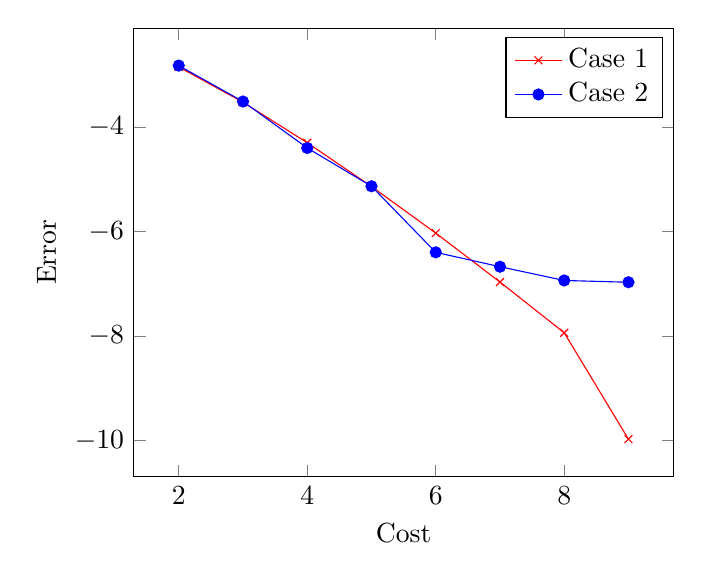
\begin{tikzpicture}
	\begin{axis}[
		xlabel=Cost,
		ylabel=Error]
	\addplot[color=red,mark=x] coordinates {
		(2,-2.8559703)
		(3,-3.5301677)
		(4,-4.3050655)
		(5,-5.1413136)
		(6,-6.0322865)
		(7,-6.9675052)
		(8,-7.9377747)
		(9,-9.9717663)
		};
	\addplot[color=blue,mark=*] coordinates {
		(2,-2.83)
		(3,-3.5167)
		(4,-4.4050)
		(5,-5.137)
		(6,-6.4)
		(7,-6.6750)
		(8,-6.9377)
		(9,-6.9717)
		};
	\legend{Case 1,Case 2}
	\end{axis}
\end{tikzpicture}

\caption{Two plots in the same axis. A legend can be generated using the \texttt{\textbackslash legend{}}-command.}
\label{fig:twoplots}
\end{figure}

\begin{lstlisting}
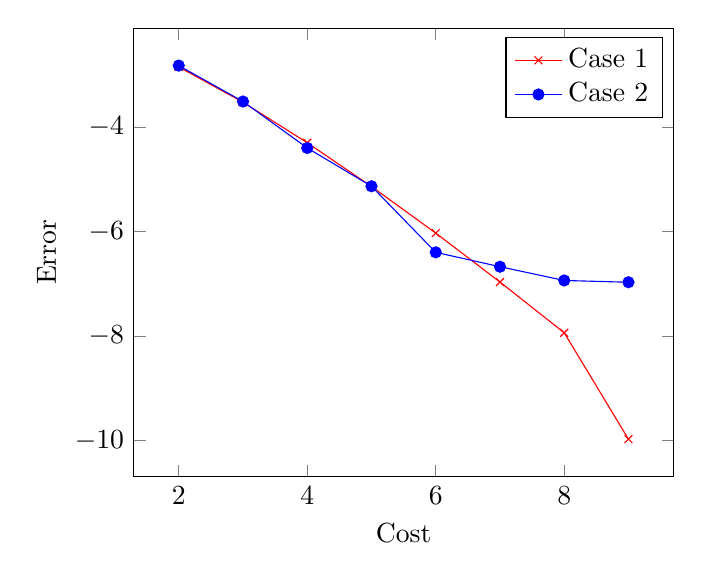
\begin{tikzpicture}
	\begin{axis}[
		xlabel=Cost,
		ylabel=Error]
	\addplot[color=red,mark=x] coordinates {
		(2,-2.8559703)
		(3,-3.5301677)
		(4,-4.3050655)
		(5,-5.1413136)
		(6,-6.0322865)
		(7,-6.9675052)
		(8,-7.9377747)
		(9,-9.9717663)
	};
	\addplot[color=blue,mark=*] coordinates {
		(2,-2.83)
		(3,-3.5167)
		(4,-4.4050)
		(5,-5.137)
		(6,-6.4)
		(7,-6.6750)
		(8,-6.9377)
		(9,-6.9717)
	};
	\legend{Case 1,Case 2}
	\end{axis}
\end{tikzpicture}
\end{lstlisting}

\subsection{Logarithmic plots}
Logarithmic plots show $\log x$ versus $\log y$  (or just one logarithmic axis) as in figure~\ref{fig:firstloglog}. \PGFPlots\ always uses the natural logarithm, i.e. basis $e\approx2.718$. Now, the axis description also contains minor ticks and the labels are placed at $10^i$.
\begin{figure}
\centering
	\begin{tikzpicture}
	\begin{loglogaxis}[xlabel=Cost,ylabel=Gain]
	\addplot[color=red,mark=x] coordinates {
		(10,100)
		(20,150)
		(40,225)
		(80,340)
		(160,510)
		(320,765)
		(640,1150)
	};
	\end{loglogaxis}
	\end{tikzpicture}

\caption{A double--logarithmic plot.}
\label{fig:firstloglog}
\end{figure}
\begin{lstlisting}
\begin{tikzpicture}
\begin{loglogaxis}[xlabel=Cost,ylabel=Gain]
\addplot[color=red,mark=x] coordinates {
	(10,100)
	(20,150)
	(40,225)
	(80,340)
	(160,510)
	(320,765)
	(640,1150)
};
\end{loglogaxis}
\end{tikzpicture}
\end{lstlisting}
A common application is to visualise scientific data. This is often provided in the format $1.42\cdot10^4$, usually written as 1.42e+04. An example is shown in the following listing and in figure~\ref{fig:example:sci:loglog}.
\begin{figure}
\centering
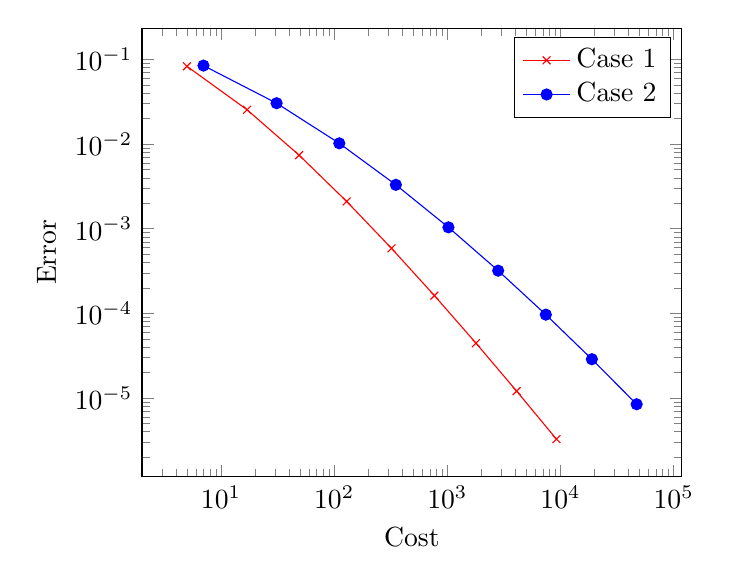
\begin{tikzpicture}
	\begin{loglogaxis}[
		xlabel=Cost,
		ylabel=Error]
	\addplot[color=red,mark=x] coordinates {
		(5,		8.31160034e-02)
		(17,	2.54685628e-02)
		(49,	7.40715288e-03)
		(129,	2.10192154e-03)
		(321,	5.87352989e-04)
		(769,	1.62269942e-04)
		(1793,	4.44248889e-05)
		(4097,	1.20714122e-05)
		(9217,	3.26101452e-06)
	};

	\addplot[color=blue,mark=*] coordinates {
		(7,		8.47178381e-02)
		(31,	3.04409349e-02)
		(111,	1.02214539e-02)
		(351,	3.30346265e-03)
		(1023,	1.03886535e-03)
		(2815,	3.19646457e-04)
		(7423,	9.65789766e-05)
		(18943,	2.87339125e-05)
		(47103,	8.43749881e-06)
	};
	\legend{Case 1,Case 2}
	\end{loglogaxis}
\end{tikzpicture}

\caption{A double--logarithmic plot using scientific notation.}
\label{fig:example:sci:loglog}
\end{figure}

\begin{lstlisting}
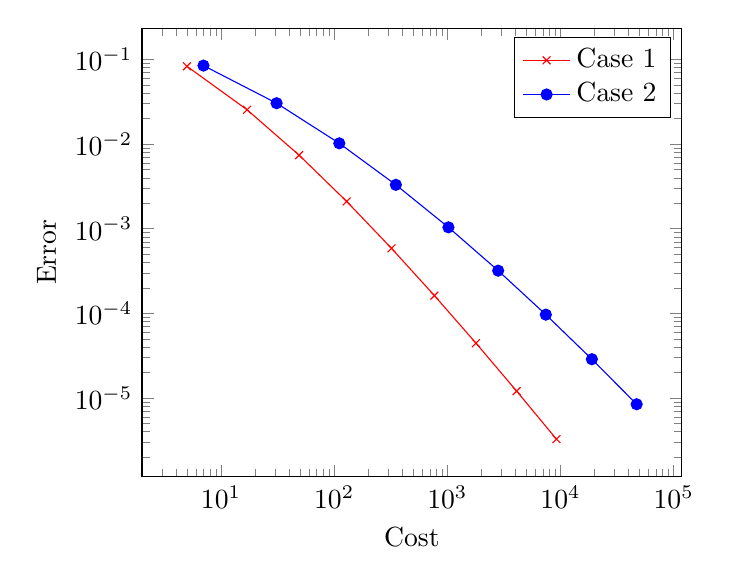
\begin{tikzpicture}
	\begin{loglogaxis}[
		xlabel=Cost,
		ylabel=Error]
	\addplot[color=red,mark=x] coordinates {
		(5,		8.31160034e-02)
		(17,	2.54685628e-02)
		(49,	7.40715288e-03)
		(129,	2.10192154e-03)
		(321,	5.87352989e-04)
		(769,	1.62269942e-04)
		(1793,	4.44248889e-05)
		(4097,	1.20714122e-05)
		(9217,	3.26101452e-06)
	};

	\addplot[color=blue,mark=*] coordinates {
		(7,		8.47178381e-02)
		(31,	3.04409349e-02)
		(111,	1.02214539e-02)
		(351,	3.30346265e-03)
		(1023,	1.03886535e-03)
		(2815,	3.19646457e-04)
		(7423,	9.65789766e-05)
		(18943,	2.87339125e-05)
		(47103,	8.43749881e-06)
	};
	\legend{Case 1,Case 2}
	\end{loglogaxis}
\end{tikzpicture}
\end{lstlisting}
Besided the environment ``\texttt{loglogaxis}'' you can use
\begin{itemize}
	\item \lstinline!\begin{axis}...\end{axis}! for normal plots,
	\item \lstinline!\begin{semilogxaxis}...\end{semilogxaxis}! for plots which have a normal~$y$ axis and a logarithmic~$x$ axis,
	\item \lstinline!\begin{semilogyaxis}...\end{semilogyaxis}! the same with $x$~and~$y$ switched,
	\item \lstinline!\begin{loglogaxis}...\end{loglogaxis}! for double--logarithmic plots.
\end{itemize}
You can also use
\begin{lstlisting}
	\begin{axis}[xmode=normal,ymode=log]
	...
	\end{axis}
\end{lstlisting}
which is the same as \lstinline!\begin{semilogyaxis}...\end{semilogyaxis}!. Example:
\begin{lstlisting}
\begin{tikzpicture}
	\begin{semilogyaxis}[xlabel=Index,ylabel=Value]
	\addplot[color=blue,mark=*] coordinates {
		(1,8)
		(2,16)
		(3,32)
		(4,64)
		(5,128)
		(6,256)
		(7,512)
	};
	\end{semilogyaxis}
\end{tikzpicture}
\end{lstlisting}
see figure~\ref{fig:semilogy}.
\begin{figure}
\centering
\begin{tikzpicture}
	\begin{semilogyaxis}[xlabel=Index,ylabel=Value]
	\addplot[color=blue,mark=*] coordinates {
		(1,8)
		(2,16)
		(3,32)
		(4,64)
		(5,128)
		(6,256)
		(7,512)
	};
	\end{semilogyaxis}
\end{tikzpicture}

\caption{A semi--logarithmic plot.}
\label{fig:semilogy}
\end{figure}

\subsection{Cycling line styles}
You can skip the style arguments for \lstinline!\addplot[...]! or \lstinline!\addplot[...]! to determine plot specifications from a predefined list:
\begin{figure}
\centering
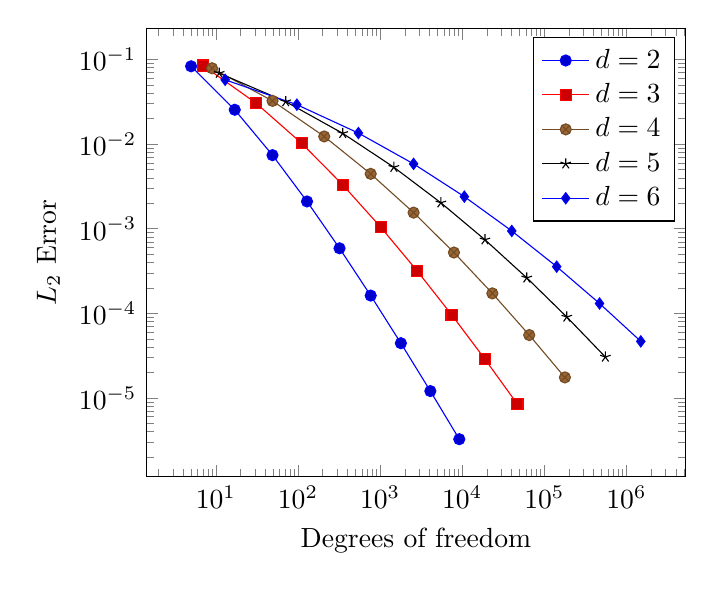
\begin{tikzpicture}
	\begin{loglogaxis}[
		xlabel={Degrees of freedom},
		ylabel={$L_2$ Error}
	]
	\addplot coordinates {
		(5,		8.312e-02)
		(17,	2.547e-02)
		(49,	7.407e-03)
		(129,	2.102e-03)
		(321,	5.874e-04)
		(769,	1.623e-04)
		(1793,	4.442e-05)
		(4097,	1.207e-05)
		(9217,	3.261e-06)
	};

	\addplot coordinates {
		(7,		8.472e-02)
		(31,	3.044e-02)
		(111,	1.022e-02)
		(351,	3.303e-03)
		(1023,	1.039e-03)
		(2815,	3.196e-04)
		(7423,	9.658e-05)
		(18943,	2.873e-05)
		(47103,	8.437e-06)
	};

	\addplot coordinates {
		(9,		7.881e-02)
		(49,	3.243e-02)
		(209,	1.232e-02)
		(769,	4.454e-03)
		(2561,	1.551e-03)
		(7937,	5.236e-04)
		(23297,	1.723e-04)
		(65537,	5.545e-05)
		(178177,	1.751e-05)
	};

	\addplot coordinates {
		(11,	6.887e-02)
		(71,	3.177e-02)
		(351,	1.341e-02)
		(1471,	5.334e-03)
		(5503,	2.027e-03)
		(18943,	7.415e-04)
		(61183,	2.628e-04)
		(187903,	9.063e-05)
		(553983,	3.053e-05)
	};

	\addplot coordinates {
		(13,	5.755e-02)
		(97,	2.925e-02)
		(545,	1.351e-02)
		(2561,	5.842e-03)
		(10625,	2.397e-03)
		(40193,	9.414e-04)
		(141569,	3.564e-04)
		(471041,	1.308e-04)
		(1496065,	4.670e-05)
	};
	\legend{$d=2$,$d=3$,$d=4$,$d=5$,$d=6$}
	\end{loglogaxis}
\end{tikzpicture}

\caption{Predefined line/marker combinations.}
\label{fig:predefined:plotspec}
\end{figure}

\begin{lstlisting}
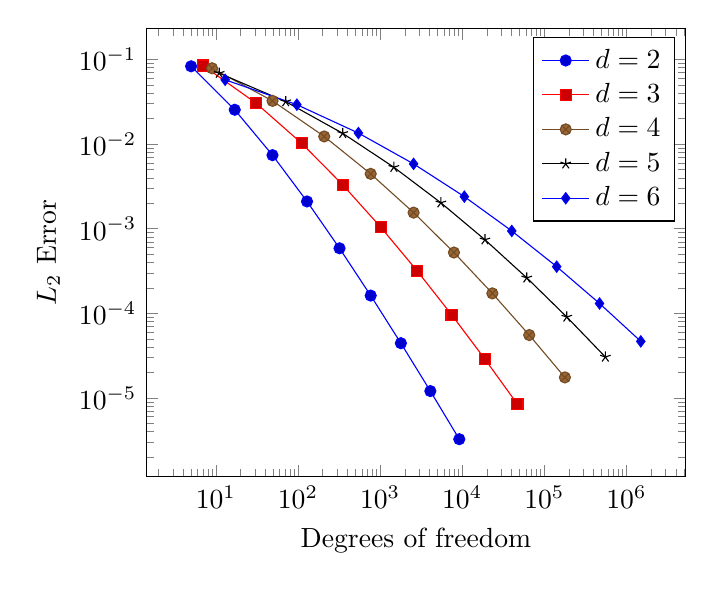
\begin{tikzpicture}
	\begin{loglogaxis}[
		xlabel={Degrees of freedom},
		ylabel={$L_2$ Error}
	]
	\addplot coordinates {
		(5,		8.312e-02)
		(17,	2.547e-02)
		(49,	7.407e-03)
		(129,	2.102e-03)
		(321,	5.874e-04)
		(769,	1.623e-04)
		(1793,	4.442e-05)
		(4097,	1.207e-05)
		(9217,	3.261e-06)
	};

	\addplot coordinates {
		(7,		8.472e-02)
		(31,	3.044e-02)
		(111,	1.022e-02)
		(351,	3.303e-03)
		(1023,	1.039e-03)
		(2815,	3.196e-04)
		(7423,	9.658e-05)
		(18943,	2.873e-05)
		(47103,	8.437e-06)
	};

	\addplot coordinates {
		(9,		7.881e-02)
		(49,	3.243e-02)
		(209,	1.232e-02)
		(769,	4.454e-03)
		(2561,	1.551e-03)
		(7937,	5.236e-04)
		(23297,	1.723e-04)
		(65537,	5.545e-05)
		(178177,	1.751e-05)
	};

	\addplot coordinates {
		(11,	6.887e-02)
		(71,	3.177e-02)
		(351,	1.341e-02)
		(1471,	5.334e-03)
		(5503,	2.027e-03)
		(18943,	7.415e-04)
		(61183,	2.628e-04)
		(187903,	9.063e-05)
		(553983,	3.053e-05)
	};

	\addplot coordinates {
		(13,	5.755e-02)
		(97,	2.925e-02)
		(545,	1.351e-02)
		(2561,	5.842e-03)
		(10625,	2.397e-03)
		(40193,	9.414e-04)
		(141569,	3.564e-04)
		(471041,	1.308e-04)
		(1496065,	4.670e-05)
	};
	\legend{$d=2$,$d=3$,$d=4$,$d=5$,$d=6$}
	\end{loglogaxis}
\end{tikzpicture}
\end{lstlisting}

The result is shown in figure~\ref{fig:predefined:plotspec}. You can modify the list, see the reference below.

\subsection{Scaling plots}
You can use any of the \Tikz\ options to modify the appearance. For example the effect of the ``\texttt{scale}'' transformation is shown in figures \ref{fig:scale1}~and~\ref{fig:scale2}.

\begin{figure}
\begin{minipage}[c]{7.1cm}%
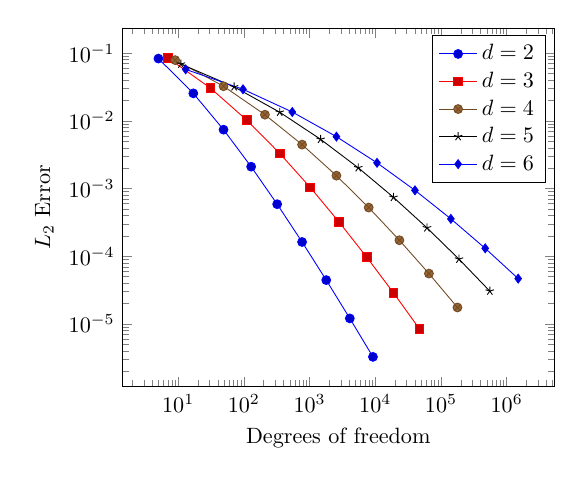
\begin{tikzpicture}[scale=0.8]
	\begin{loglogaxis}[
		xlabel={Degrees of freedom},
		ylabel={$L_2$ Error}
	]
	\addplot coordinates {
		(5,		8.312e-02)
		(17,	2.547e-02)
		(49,	7.407e-03)
		(129,	2.102e-03)
		(321,	5.874e-04)
		(769,	1.623e-04)
		(1793,	4.442e-05)
		(4097,	1.207e-05)
		(9217,	3.261e-06)
	};

	\addplot coordinates {
		(7,		8.472e-02)
		(31,	3.044e-02)
		(111,	1.022e-02)
		(351,	3.303e-03)
		(1023,	1.039e-03)
		(2815,	3.196e-04)
		(7423,	9.658e-05)
		(18943,	2.873e-05)
		(47103,	8.437e-06)
	};

	\addplot coordinates {
		(9,		7.881e-02)
		(49,	3.243e-02)
		(209,	1.232e-02)
		(769,	4.454e-03)
		(2561,	1.551e-03)
		(7937,	5.236e-04)
		(23297,	1.723e-04)
		(65537,	5.545e-05)
		(178177,	1.751e-05)
	};

	\addplot coordinates {
		(11,	6.887e-02)
		(71,	3.177e-02)
		(351,	1.341e-02)
		(1471,	5.334e-03)
		(5503,	2.027e-03)
		(18943,	7.415e-04)
		(61183,	2.628e-04)
		(187903,	9.063e-05)
		(553983,	3.053e-05)
	};

	\addplot coordinates {
		(13,	5.755e-02)
		(97,	2.925e-02)
		(545,	1.351e-02)
		(2561,	5.842e-03)
		(10625,	2.397e-03)
		(40193,	9.414e-04)
		(141569,	3.564e-04)
		(471041,	1.308e-04)
		(1496065,	4.670e-05)
	};
	\legend{$d=2$,$d=3$,$d=4$,$d=5$,$d=6$}
	\end{loglogaxis}
\end{tikzpicture}
\end{minipage}%
\hfill
\begin{minipage}[c]{8cm}%
\begin{lstlisting}
\begin{tikzpicture}[scale=0.8]
\begin{loglogaxis}
...
\end{loglogaxis}
\end{tikzpicture}
\end{lstlisting}
\end{minipage}
\caption{An example of a scaled plot.}
\label{fig:scale1}
\end{figure}

\begin{figure}
\centering
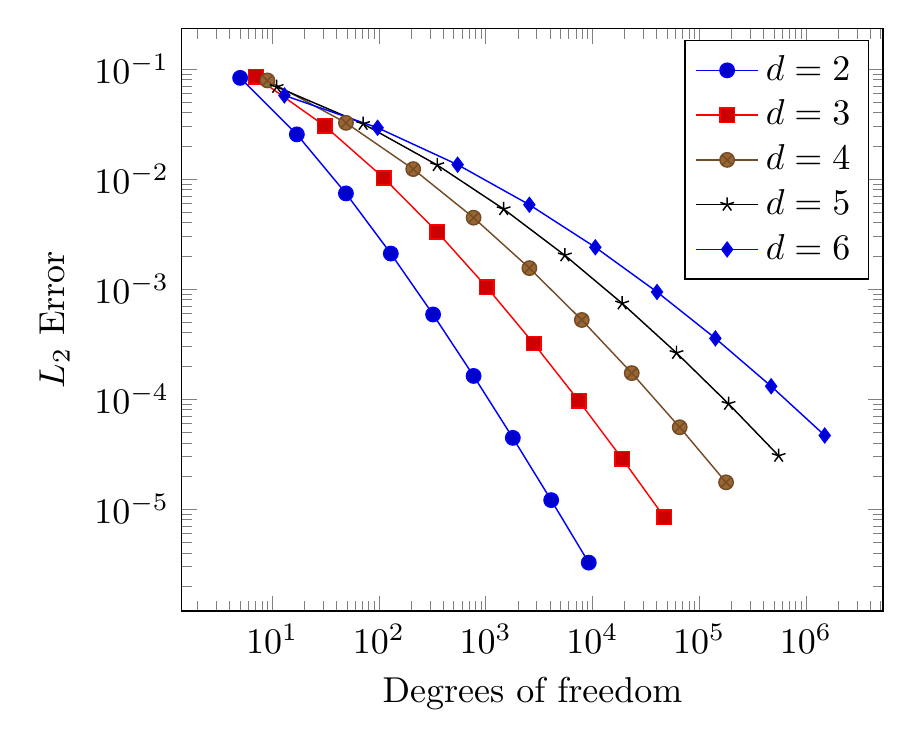
\begin{tikzpicture}[scale=1.3]
	\begin{loglogaxis}[
		xlabel={Degrees of freedom},
		ylabel={$L_2$ Error}
	]
	\addplot coordinates {
		(5,		8.312e-02)
		(17,	2.547e-02)
		(49,	7.407e-03)
		(129,	2.102e-03)
		(321,	5.874e-04)
		(769,	1.623e-04)
		(1793,	4.442e-05)
		(4097,	1.207e-05)
		(9217,	3.261e-06)
	};

	\addplot coordinates {
		(7,		8.472e-02)
		(31,	3.044e-02)
		(111,	1.022e-02)
		(351,	3.303e-03)
		(1023,	1.039e-03)
		(2815,	3.196e-04)
		(7423,	9.658e-05)
		(18943,	2.873e-05)
		(47103,	8.437e-06)
	};

	\addplot coordinates {
		(9,		7.881e-02)
		(49,	3.243e-02)
		(209,	1.232e-02)
		(769,	4.454e-03)
		(2561,	1.551e-03)
		(7937,	5.236e-04)
		(23297,	1.723e-04)
		(65537,	5.545e-05)
		(178177,	1.751e-05)
	};

	\addplot coordinates {
		(11,	6.887e-02)
		(71,	3.177e-02)
		(351,	1.341e-02)
		(1471,	5.334e-03)
		(5503,	2.027e-03)
		(18943,	7.415e-04)
		(61183,	2.628e-04)
		(187903,	9.063e-05)
		(553983,	3.053e-05)
	};

	\addplot coordinates {
		(13,	5.755e-02)
		(97,	2.925e-02)
		(545,	1.351e-02)
		(2561,	5.842e-03)
		(10625,	2.397e-03)
		(40193,	9.414e-04)
		(141569,	3.564e-04)
		(471041,	1.308e-04)
		(1496065,	4.670e-05)
	};
	\legend{$d=2$,$d=3$,$d=4$,$d=5$,$d=6$}
	\end{loglogaxis}
\end{tikzpicture}

\begin{lstlisting}
			\begin{tikzpicture}[scale=1.3]
			\begin{loglogaxis}
			...
			\end{loglogaxis}
			\end{tikzpicture}
\end{lstlisting}
\caption{The effect of a ``\texttt{scale}'' transformation by~$30\%$.}
\label{fig:scale2}
\end{figure}

You can scale plots either using the \texttt{width=5cm} and/or \texttt{height=3cm} options or by setting the dimension for each unit coordinate as is shown in figure~\ref{fig:scale:units}.

More examples can be found in section~\ref{sec:examples}.

\begin{figure}
\centering
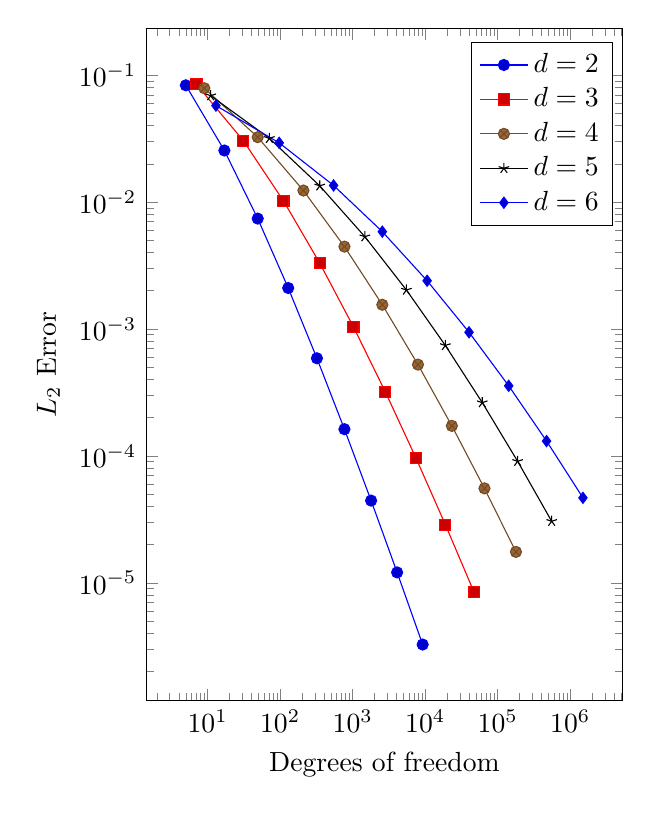
\begin{tikzpicture}
	\begin{loglogaxis}[%
		x=0.4cm,y=0.7cm,
		xlabel={Degrees of freedom},
		ylabel={$L_2$ Error}
	]
	\addplot coordinates {
		(5,		8.312e-02)
		(17,	2.547e-02)
		(49,	7.407e-03)
		(129,	2.102e-03)
		(321,	5.874e-04)
		(769,	1.623e-04)
		(1793,	4.442e-05)
		(4097,	1.207e-05)
		(9217,	3.261e-06)
	};

	\addplot coordinates {
		(7,		8.472e-02)
		(31,	3.044e-02)
		(111,	1.022e-02)
		(351,	3.303e-03)
		(1023,	1.039e-03)
		(2815,	3.196e-04)
		(7423,	9.658e-05)
		(18943,	2.873e-05)
		(47103,	8.437e-06)
	};

	\addplot coordinates {
		(9,		7.881e-02)
		(49,	3.243e-02)
		(209,	1.232e-02)
		(769,	4.454e-03)
		(2561,	1.551e-03)
		(7937,	5.236e-04)
		(23297,	1.723e-04)
		(65537,	5.545e-05)
		(178177,	1.751e-05)
	};

	\addplot coordinates {
		(11,	6.887e-02)
		(71,	3.177e-02)
		(351,	1.341e-02)
		(1471,	5.334e-03)
		(5503,	2.027e-03)
		(18943,	7.415e-04)
		(61183,	2.628e-04)
		(187903,	9.063e-05)
		(553983,	3.053e-05)
	};

	\addplot coordinates {
		(13,	5.755e-02)
		(97,	2.925e-02)
		(545,	1.351e-02)
		(2561,	5.842e-03)
		(10625,	2.397e-03)
		(40193,	9.414e-04)
		(141569,	3.564e-04)
		(471041,	1.308e-04)
		(1496065,	4.670e-05)
	};
	\legend{$d=2$,$d=3$,$d=4$,$d=5$,$d=6$}
	\end{loglogaxis}
\end{tikzpicture}%

\begin{lstlisting}
		\begin{tikzpicture}
		\begin{loglogaxis}[x=0.4cm,y=0.7cm,...]
		...
		\end{loglogaxis}
		\end{tikzpicture}
\end{lstlisting}
\caption{The result of setting the unit vector for~$x$ to~0.4cm and for~$y$ to~0.7cm.}
\label{fig:scale:units}
\end{figure}

